\chapter{Analisis}
Pada bab ini akan dipaparkan analisis yang dilakukan dalam pembuatan aplikasi
ini. Bagaimana data XML didapatkan dari situs \url{www.openstreetmap.org}
yang akan dibahas pada subbab \ref{ssec:analisis_osm} dan membacanya
menggunakan beberapa fungsi javascript yang akan dibahas
pada subbab \ref{ssec:analisis_js}. Setelah itu, data tersebut disimpan atau
dikonversi ke dalam bentuk graf sehingga dapat digunakan algoritma dijkstra untuk mencari rute 
terpendek dari satu node ke node lain. Berdasarkan informasi yang telah diolah,
maka dapat dibuat visualisasi data atau informasi tersebut menggunakan Google
Maps Javascript API. Pada akhir bab ini, juga akan dibahas mengenai \textit{use
case diagram} dan skenario untuk memperjelas apa saja yang dapat dilakukan oleh
\textit{user} pada aplikasi ini.

\section{Analisis OpenStreetMap} \label{ssec:analisis_osm}
OpenStreetMap adalah portal peta terbuka yang menyediakan data dalam bentuk peta
ataupun dokumen XML. Aplikasi yang dibuat akan berbasis OpenStreetMap, hal ini
berarti aplikasi yang dibuat akan menggunakan data yang diperoleh dari situs
\url{www.openstreetmap.org}. Untuk mendapatkan data peta pada situs
OpenStreetMap, user harus mengunjungi situs tersebut dan menggunakan fitur
\textit{export}. Data yang digunakan adalah data peta yang berbentuk
dokumen XML atau biasa disebut dengan OSMXML. Selanjutnya, informasi yang
terkandung di dalam dokumen OSMXML tersebut akan diproses untuk mengetahui node dan edge
pada peta. Informasi tersebut akan diubah ke dalam bentuk graf yang akan
diproses lebih lanjut menggunakan algoritma dijkstra untuk mengetahui jarak
terpendek dari satu node ke node lain.

\subsection{Langkah-Langkah Pengambilan Data OSMXML}
Berikut ini adalah langkah-langkah pengambilan data OSMXML yang akan digunakan:
\begin{enumerate}
  \item Mengunjungi situs \url{www.openstreetmap.org}.
  
  \item Menggunakan fitur \textit{search} untuk mencari area lokasi yang
  diinginkan. penggunaan fitur ini dapat dilihat pada Gambar
  \ref{fig:osmsearch_analisis} .
\begin{figure}[h]
\centering
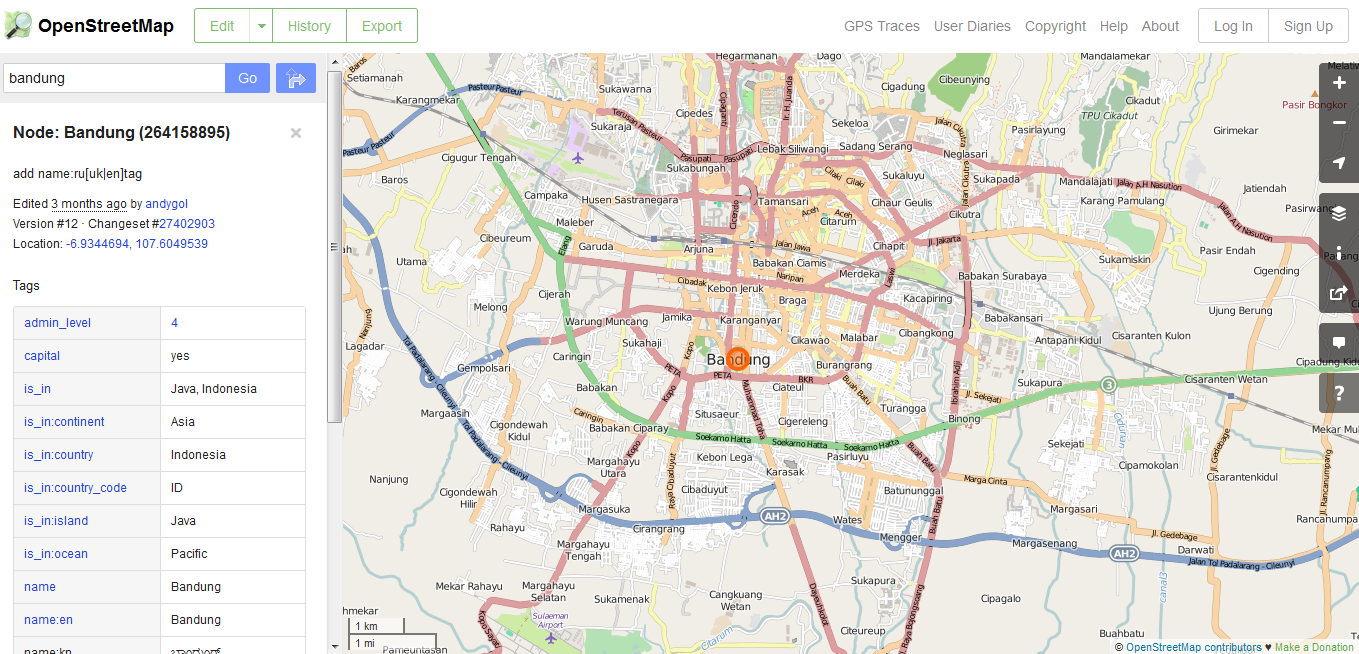
\includegraphics[scale=0.4]{Gambar/osmsearch_analisis}
\caption[Fitur search pada situs OpenStreetMap]{Fitur search pada situs
OpenStreetMap}
\label{fig:osmsearch_analisis}
\end{figure}
  
  \item Menggunakan fitur \textit{export} untuk mengunduh data dalam
  bentuk dokumen XML. penggunaan fitur ini dapat dilihat pada Gambar
  \ref{fig:osmxml_analisis}.
\begin{figure}[h]
\centering
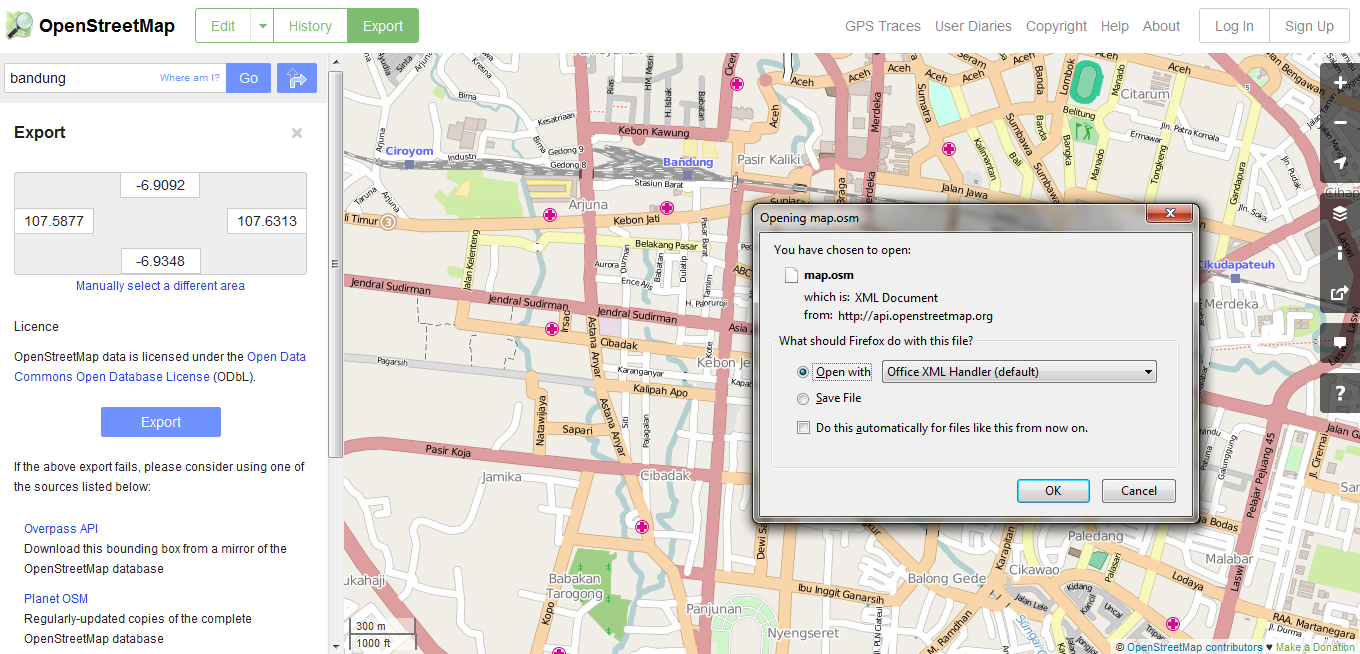
\includegraphics[scale=0.4]{Gambar/osmxml_analisis}
\caption[Fitur search pada situs OpenStreetMap]{Fitur \textit{export} pada situs
OpenStreetMap}
\label{fig:osmxml_analisis}
\end{figure}
\end{enumerate}

\subsection{OSMXML}
Sesuai dengan pembahasan pada subbab \ref{ssec:osmxml}, OSMXML merupakan dokumen
XML yang mengandung data-data peta OpenStreetMap. Contoh data yang sudah diunduh
dapat dilihat di bawah ini.
\begin{lstlisting}
<?xml version="1.0" encoding="UTF-8"?>
<osm version="0.6" generator="CGImap 0.3.3 (29805 thorn-03.openstreetmap.org)" copyright="OpenStreetMap and contributors" attribution="http://www.openstreetmap.org/copyright" license="http://opendatacommons.org/licenses/odbl/1-0/">
 <bounds minlat="-6.9076500" minlon="107.5961800" maxlat="-6.9044500" maxlon="107.6016300"/>
 <node id="25418868" visible="true" version="6" changeset="27915808" timestamp="2015-01-04T17:54:58Z" user="isonpurba" uid="2552445" lat="-6.9064389" lon="107.5976351"/>
 <node id="25433683" visible="true" version="3" changeset="839915" timestamp="2009-03-21T14:18:48Z" user="adhitya" uid="7748" lat="-6.9067659" lon="107.5989458"/>
 ...
 <node id="25433687" visible="true" version="2" changeset="839915" timestamp="2009-03-21T14:18:36Z" user="adhitya" uid="7748" lat="-6.9040267" lon="107.5969508"/>
 <node id="25433688" visible="true" version="2" changeset="839915" timestamp="2009-03-21T14:18:58Z" user="adhitya" uid="7748" lat="-6.9039393" lon="107.5963723"/>
 <node id="25500626" visible="true" version="3" changeset="839915" timestamp="2009-03-21T14:22:17Z" user="adhitya" uid="7748" lat="-6.9070329" lon="107.6019401"/>
 ...
<node id="3030289971" visible="true" version="1" changeset="24892866" timestamp="2014-08-20T18:40:31Z" user="albahrimaraxsa" uid="2162153" lat="-6.9066710" lon="107.5982569"/>
 <node id="2325451442" visible="true" version="4" changeset="27916144" timestamp="2015-01-04T18:06:33Z" user="isonpurba" uid="2552445" lat="-6.9045011" lon="107.6024922"/>
 <way id="4567626" visible="true" version="4" changeset="15861148" timestamp="2013-04-25T13:56:12Z" user="mrdoggie94" uid="1331966">
  <nd ref="25433682"/>
  <nd ref="25433681"/>
  <nd ref="25433680"/>
  <tag k="avgspeed" v="15"/>
  <tag k="highway" v="residential"/>
  <tag k="name" v="Dr. Rubini"/>
 </way>
 <way id="4567634" visible="true" version="2" changeset="7821743" timestamp="2011-04-10T11:15:30Z" user="evo2mind" uid="234610">
  <nd ref="25433681"/>
  <nd ref="28802396"/>
  <tag k="avgspeed" v="15"/>
  <tag k="highway" v="residential"/>
  <tag k="name" v="Dr. Susilo"/>
 </way>
 ...
</osm>
\end{lstlisting}
Node dan way memiliki informasi penting yang akan digunakan pada aplikasi. Pada
tag node terdapat atribut id yang menunjukkan id pada setiap node, kemudian
terdapat atribut lat dan lon yang memberikan informasi titik koordinat
(\textit{latitude} dan \textit{longitude})pada node tersebut. Informasi yang
didapatkan akan disimpan ke dalam bentuk node pada graf. Tag way akan
menunjukkan hubungan pada node-node yang terdapat pada dokumen, dan akan
disimpan sebagai edge pada graf. Selain itu, tag way tidak hanya memberikan
informasi jalan raya atau jalan besar saja, tetapi juga beberapa elemen peta
lain seperti area sekeliling bangunan atau area sekitar tempat parkir. Maka dari
itu, diperlukan \textit{filter} pada tag way, karena hanya informasi jalan raya
atau jalan besar saja yang diperlukan oleh aplikasi. Data atau dokumen XML yang
telah diperoleh, selanjutnya akan dibaca menggunakan javascript yang akan
dibahas pada subbab \ref{ssec:analisis_js}.

\section{Analisis Javascript} \label{ssec:analisis_js}
Javascript diperlukan untuk membaca dokumen XML, sehingga seluruh informasi yang
diperlukan dapat diubah ke dalam bentuk graf yang akan diproses lebih lanjut.
XMLHttpRequest adalah salah satu objek pada javascript yang dapat digunakan 
untuk mendapatkan \textit{file} XML. Berikut ini adalah contoh kode
program yang akan digunakan untuk mendapatkan \textit{file} XML:
\begin{verbatim}
xmlhttp=new XMLHttpRequest();
xmlhttp.open("GET","map.xml",false);
xmlhttp.send();
xmlDoc=xmlhttp.responseXML;
\end{verbatim}
Setelah mendapatkan \textit{file} XML, diperlukan XML DOM untuk membaca
informasi yang diperlukan pada dokumen XML. Berikut ini adalah contoh kode
program yang akan digunakan:
\begin{verbatim}
var node = xmlDoc.getElementsByTagName("node");
var way = xmlDoc.getElementsByTagName("way");

var id_node = node[0].getAttribute('id');
\end{verbatim}
Di bawah ini adalah contoh kode program yang digunakan untuk menampilkan
informasi dari dokumen XML dalam bentuk tabel:
\begin{lstlisting}
<html>
<head>
<style>
table, th, td {
    border: 1px solid black;
    border-collapse:collapse;
}
th, td {
    padding: 5px;
}
</style>
</head>
<body>
<script>
xmlhttp=new XMLHttpRequest();
xmlhttp.open("GET","map.xml",false);
xmlhttp.send();
xmlDoc=xmlhttp.responseXML;

document.write("<div style='float: left'>");
document.write("<table><tr><th>Node</th><th>Id</th><th>Latitude</th><th>Longitude</th></tr>");
document.write("<caption>Node</caption>");
var node=xmlDoc.getElementsByTagName("node");
for (ct=0;ct<node.length;ct++)
  {
  document.write("<tr><td>");
  document.write(ct);
  document.write("</td><td>");
  document.write(node[ct].getAttribute('id'));
  document.write("</td><td>");
  document.write(node[ct].getAttribute('lat'));
  document.write("</td><td>");
  document.write(node[ct].getAttribute('lon'));
  document.write("</td></tr>");
  }
document.write("</table>");
document.write("</div>");

function isHighway(way,index){
	var tag = way[index].getElementsByTagName("tag");
	for (hg=0;hg<tag.length;hg++)
	{
		if(tag[hg].getAttribute('k') == "highway"){
			return true;
		}
	}
	return false;
}

document.write("<div style='margin-left: 20px;float: left'>");
document.write("<table><tr><th>Way</th><th>Id Way</th><th>Edge</th><th>Id Node 1</th><th>Id Node 2</th></tr>");
document.write("<caption>Edge</caption>");
var way = xmlDoc.getElementsByTagName("way");
var nd;
for (i=0;i<way.length;i++)
{
	nd = way[i].getElementsByTagName("nd");
	if(isHighway(way,i)){
		for (j=0;j<nd.length-1;j++)
		{
			document.write("<tr><td>");
			document.write(i);
			document.write("</td><td>");
			document.write(way[i].getAttribute('id'));
			document.write("</td><td>");
			document.write(j);
			document.write("</td><td>");
			document.write(nd[j].getAttribute('ref'));
			document.write("</td><td>");
			document.write(nd[j+1].getAttribute('ref'));	
			document.write("</td></tr>");
		}
	}
}
document.write("</div>");
</script>
</body>
</html>
\end{lstlisting}
Hasil dari kode program di atas dapat dilihat pada Gambar \ref{fig:xml_parsing}.
\begin{figure}[h]
\centering
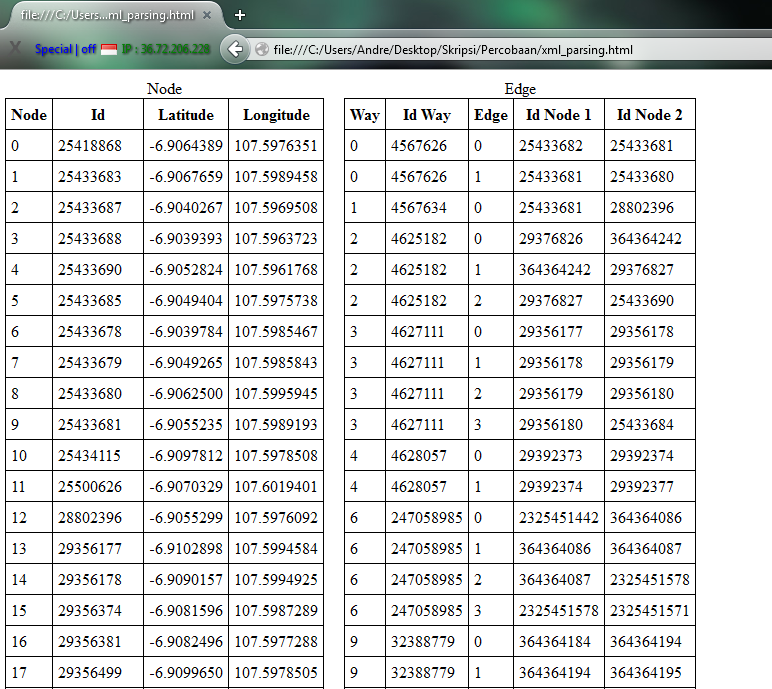
\includegraphics[scale=0.5]{Gambar/xml_parsing}
\caption[Parsing XML menggunakan Javascript]{Parsing XML menggunakan
Javascript}
\label{fig:xml_parsing}
\end{figure}

Pada Gambar \ref{fig:xml_parsing} dapat dilihat terdiri dari dua tabel yang
menunjukkan informasi node dan edge yang sudah dibaca. Tabel node menunjukkan
atribut penting yang akan digunakan yaitu id node, \textit{latitude}, dan
\textit{longitude}. Sedangkan tabel edge menujukkan informasi yang didapatkan
dari tag way yang sudah dilakukan \textit{filter}, yaitu hanya tag highway saja
yang akan digunakan. Pada tabel edge terdapat informasi penting yang
akan digunakan, yaitu id way, id node pertama, dan id node kedua. Informasi yang
sudah didapatkan, selanjutnya akan dimodelkan ke dalam bentuk graf yang akan
dibahas pada subbab \ref{ssec:analisis_graf}.


\section{Pemodelan OSMXML Menjadi Graf} \label{ssec:analisis_graf}
Pada subbab \ref{ssec:analisis_js}, dokumen OSMXML sudah dibaca dan tahap
selanjutnya adalah memodelkan data OSMXML tersebut ke dalam bentuk graf. Seperti
yang sudah diketahui, graf terdiri dari node dan edge. Informasi node dan edge
yang sudah didapatkan akan dimodelkan ke dalam bentuk graf berarah, hal ini
karena jalan yang menghubungkan node-node tersebut memiliki arah, baik searah
maupun dua arah. Untuk merepresentasikan graf tersebut akan digunakan
\textit{adjacency list}. Di bawah ini adalah contoh kode program yang digunakan
untuk memodelkan dokumen OSMXML menjadi graf:
\begin{lstlisting}
 <!DOCTYPE html>
<html>
<head>
</head>
<body>
<script>
xmlhttp=new XMLHttpRequest();
xmlhttp.open("GET","map.xml",false);
xmlhttp.send();
xmlDoc=xmlhttp.responseXML;

function Neighbor(vnum, nbr){
    this.vertexNum = vnum;
    this.next = nbr;
}

function Node(id, neighbors){
    this.id = id;
    this.adjList = neighbors;
}

function isHighway(way,index){
	var tag = way[index].getElementsByTagName("tag");
	for (hg=0;hg<tag.length;hg++)
	{
		if(tag[hg].getAttribute('k') == "highway"){
			return true;
		}
	}
	return false;
}

function indexForName(adjLists,id) {
		for (var i=0; i < adjLists.length; i++){
			if (adjLists[i].id == id){
				return i;
			}
		}
		return -1;
	}

function Graph(node,way){
	var adjLists = [];
	var nd;
	
	for(v=0; v < node.length; v++){
		adjLists.push(new Node(node[v].getAttribute('id'),null));
	}
	
	for (i=0;i<way.length;i++)
	{
		nd = way[i].getElementsByTagName("nd");
		if(isHighway(way,i)){
			for (j=0;j<nd.length-1;j++)
			{
				v1 = indexForName(adjLists,nd[j].getAttribute('ref'));
				v2 = indexForName(adjLists,nd[j+1].getAttribute('ref'));

				adjLists[v1].adjList = new Neighbor(v2, adjLists[v1].adjList);
				adjLists[v2].adjList = new Neighbor(v1, adjLists[v2].adjList);
			}
		}
	}	
	return adjLists;
}

var node = xmlDoc.getElementsByTagName("node");
var way = xmlDoc.getElementsByTagName("way");

var list = new Graph(node,way);

for (j=0; j < list.length; j++){
	document.write(j);
	for (nbr=list[j].adjList; nbr != null;nbr=nbr.next) {
		document.write("---->");
		document.write('('+nbr.vertexNum+')');
	}
	document.write("<br>");
}

</script>
</body>
</html> 
\end{lstlisting}
Hasil dari kode program di atas dapat dilihat pada Gambar
\ref{fig:graf_analisis}.
\begin{figure}[h]
\centering
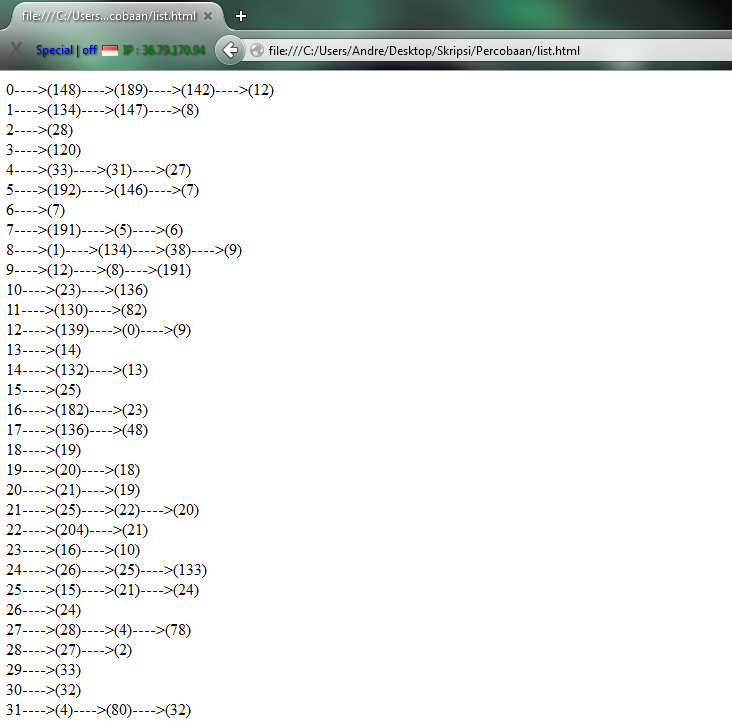
\includegraphics[scale=0.5]{Gambar/graf_analisis}
\caption[Pemodelan OSMXML menjadi Graf]{Pemodelan OSMXML menjadi Graf}
\label{fig:graf_analisis}
\end{figure}
Pada Gambar \ref{fig:graf_analisis}, data pada OSMXML sudah dimodelkan ke dalam
bentuk graf menggunakan representasi \textit{adjacency list}. Graf tersebut
selanjutnya akan divisualisasikan menggunakan Google Maps Javascript API yang
akan dibahas pada subbab \ref{ssec:analisis_gmap}.

\section{Visualisasi Graf} \label{ssec:analisis_gmap}
Data OSMXML yang sudah dimodelkan ke dalam bentuk graf, selanjutnya akan dibuat
visualisasi menggunakan Google Maps Javascript API. Peta yang akan ditampilkan
dalam bentuk \textit{roadmap}, karena peta jenis ini memberikan informasi
mengenai nama jalan, sehingga peta jenis ini lebih cocok untuk aplikasi yang
akan dikembangkan. Berikut ini adalah contoh potongan kode program untuk membuat
visualisasi graf ke dalam bentuk peta dijital menggunakan Google Maps Javascript API.
\begin{lstlisting}
function getLatByAtt(str)
{
	for (n=0;n<node.length;n++)
	{
		if(node[n].getAttribute('id') == str)
		{
			return node[n].getAttribute('lat');
		}
	}
}
function getLonByAtt(str)
{
	for (m=0;m<node.length;m++)
	{
		if(node[m].getAttribute('id') == str)
		{
			return node[m].getAttribute('lon');
		}
	}
}

function isHighway(way,index){
	var tag = way[index].getElementsByTagName("tag");
	for (hg=0;hg<tag.length;hg++)
	{
		if(tag[hg].getAttribute('k') == "highway"){
			return true;
		}
	}
	return false;
}

var currentId = 0;
var uniqueId = function() {
    return ++currentId;
}

var mapProp = {
	center:new google.maps.LatLng(-6.906845432118958,107.59851515293121),
	zoom:17,
	mapTypeId:google.maps.MapTypeId.ROADMAP
};

var map=new google.maps.Map(document.getElementById("googleMap"),mapProp);

var path = []; 
var markers = {};
var nd,marker,line,content,id;
var lat1,lon1,lat2,lon2;
var image = 'icon/dot_blue.png';

for (i=0;i<way.length;i++)
{
	nd = way[i].getElementsByTagName("nd");
	if(isHighway(way,i))
	{
		id = uniqueId();
		marker = new google.maps.Marker({
			id: id,
			position: new google.maps.LatLng(getLatByAtt(nd[0].getAttribute('ref')), getLonByAtt(nd[0].getAttribute('ref'))),
			map: map,
			icon: image,
		});
		markers[id] = marker;
		
		content = 'Id Node : '+nd[0].getAttribute('ref')+'<br>'+
			'Index Node :'+indexForName(list,nd[0].getAttribute('ref'))+'<br>'+
			'<a href="#" onclick="setAsal(\'' + id + '\')">Pilih sebagai asal</a>'+'<br>'+
			'<a href="#" onclick="setTujuan(\'' + id + '\')">Pilih sebagai tujuan</a>';
			
		addInfoWindow(marker, content);
		
		for (j=0;j<nd.length-1;j++)
		{
			id = uniqueId();
			marker = new google.maps.Marker({
				id: id,
				position: new google.maps.LatLng(getLatByAtt(nd[j+1].getAttribute('ref')), getLonByAtt(nd[j+1].getAttribute('ref'))),
				map: map,
				icon: image,
			});
			markers[id] = marker;
			
		
			content = 'Id Node : '+nd[j+1].getAttribute('ref')+'<br>'+
			'Index Node : '+indexForName(list,nd[j+1].getAttribute('ref'))+'<br>'+
			'<a href="#" onclick="setAsal(\'' + id + '\')">Pilih sebagai asal</a>'+'<br>'+
			'<a href="#" onclick="setTujuan(\'' + id + '\')">Pilih sebagai tujuan</a>';
			
			addInfoWindow(marker, content);

			line = new google.maps.Polyline({
				path: [new google.maps.LatLng(getLatByAtt(nd[j].getAttribute('ref')), getLonByAtt(nd[j].getAttribute('ref'))),
				new google.maps.LatLng(getLatByAtt(nd[j+1].getAttribute('ref')), getLonByAtt(nd[j+1].getAttribute('ref')))],
				strokeColor: "#000000",
				strokeOpacity: 1.0,
				strokeWeight: 3,
				map: map
			});
		}	
	}
}

function addInfoWindow(marker, message) {
    var infoWindow = new google.maps.InfoWindow({
        content: message
    });

	google.maps.event.addDomListener(marker, 'click', function () {
		infoWindow.open(map, marker);
	});
}
var isAsalClicked = false;
var isTujuanClicked = false;
var asal,tujuan;

function setAsal(id){
	if(!isAsalClicked){
		markers[id].setIcon('icon/dot_green.png');
		isAsalClicked = true;
		asal = id;
	}else{
		markers[asal].setIcon('icon/dot_blue.png');
		markers[id].setIcon('icon/dot_green.png');
		asal = id;
	}
}

function setTujuan(id){
	if(!isTujuanClicked){
		markers[id].setIcon('icon/dot_red.png');
		isTujuanClicked = true;
		tujuan = id;
	}else{
		markers[tujuan].setIcon('icon/dot_blue.png');
		markers[id].setIcon('icon/dot_red.png');
		tujuan = id;
	}
}
\end{lstlisting}
Hasil dari kode program di atas dapat dilihat pada Gambar
\ref{fig:visualisasi}.
\begin{figure}[h]
\centering
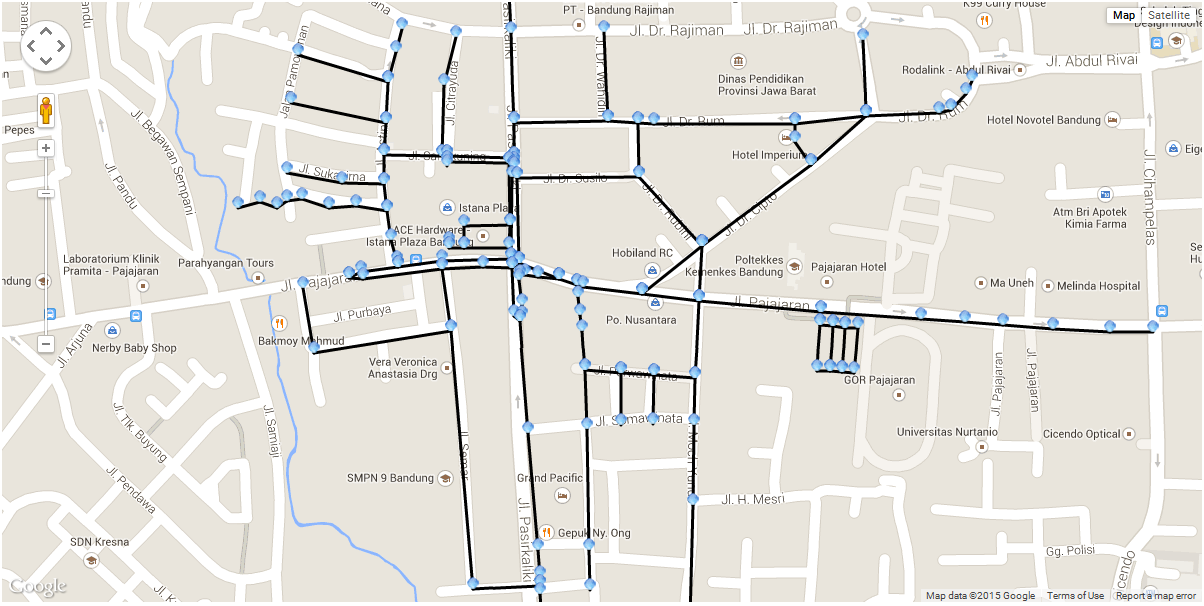
\includegraphics[scale=0.5]{Gambar/visualisasi_graf}
\caption[Visualisasi Graf]{Visualisasi Graf}
\label{fig:visualisasi}
\end{figure}

Setiap node pada graf yang sudah dilakukan \textit{filter}
akan diwakili oleh marker. Setiap marker tersebut akan memiliki \textit{info
window} yang akan memberikan informasi seperti id node, index node pada graf,
dan dua buah \textit{hyperlink} yang berfungsi untuk menjadikan marker yang
dipilih menjadi asal atau tujuan. Contoh \textit{info window} yang ditampilkan
pada peta dapat dilihat pada Gambar \ref{fig:visualisasi_infowindow}. Setiap
edge pada graf akan menjadi garis pada peta yang dibuat menggunakan \textit{polyline}.
\ref{fig:visualisasi_infowindow}.
\begin{figure}[h]
\centering
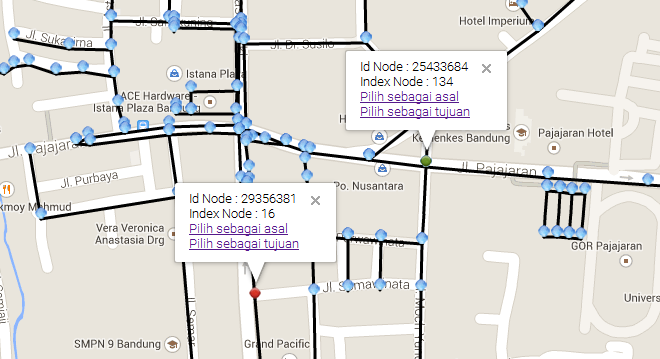
\includegraphics[scale=0.8]{Gambar/visualisasi_infowindow}
\caption[Info Window]{Info Window}
\label{fig:visualisasi_infowindow}
\end{figure}

















